
\chapter{Lecture 11}

The general rule is \emph{not} to sum quadratically all systematic uncertainties otherwise one would get a larger error the more experiment performs.
If you find deviations in systematic studies first try to understand the reason for that, then correct for the effect: including deviations into the systematical error is the last resort!
Moreover one should add only significant deviations which correspond to independent calls.\footnote{A good reference is \cite{barlow:syst_err}.}


The systematical uncertainty is a statement by experimenters about how well they understood their apparatus.
It will decrease in some cases with more data, e.g.~more precise calibration, but it \emph{cannot} shrink below a minimum uncertainty which is inherent to apparatus or method.


Once the systematical uncertainty is greater than the statistical one, acquiring more data \emph{will not} reduce the uncertainty anymore: only a better understanding of the experimental setup can improve the uncertainty.
When this is not possible, the experiment is over.


\section{Quoting results}
When you give a certain result, quote  both the systematic and statistical uncertainty separately:
\begin{equation}
	L = \SI[parse-numbers=false]{1.0 \pm 0.3 (sys) \pm 0.1 (stat)}{\meter}.
\end{equation}
The number of significant digits depends on the uncertainty.


The prescription of the \ac{pdg} are the following.
Let's consider the three highest order digit of a measurement $xyz$.
\begin{itemize}
	\item
		If $\num{100}\le xyz \le \num{354}$ then round to two significant digits, e.g.~\num{.827 \pm .119} becomes \num{.83 \pm .12};
	\item
		If $\num{355}\le xyz \le \num{949}$ then retain only one significant digit, e.g.~\num{.827 \pm .367} becomes \num{.8 \pm .4};
	\item
		If $\num{950}\le xyz \le \num{999}$ then round up to \num{1000} and keep two digits, e.g.~\num{.827 \pm .955} becomes \num{.8 \pm 1.0}.
\end{itemize}

\section{Statistical inference}

In the theory of probability, given certain \emph{known} \acp{pdf} one can obtain the probabilities for the outcomes.
The statistics deals with the inverse problem: given a data set which samples an \emph{unknown} parent \ac{pdf}, one wants to infer the parent \ac{pdf}.


Statistics can essentially be divided in two branches:
\begin{description}
	\item[Parameter estimation]
		Assume that data follow some parent \ac{pdf} (e.g.~a theoretical model), hence you can estimate its parameter by fitting;
		\Ex{Assume a Gau\ss{}ian \ac{pdf} and estimate mean and width.}

	\item[Hypothesis testing]
		Test whether data are distributed according to some parent \ac{pdf}, i.e.~in this case a theoretical model can be considered the hypothesis under test.
		\Ex{Accept of reject the hypothesis that data are Gau\ss{}ian distributed, or that an event is a signal (it may be a background noise).}
\end{description}
These branches are connected:
parameter estimation makes no sense without hypothesis on parent \ac{pdf} and often acceptance or rejection of an hypothesis on a parent \ac{pdf} requires a parameter estimation.


Sometimes ``statistics'' is referred to any function of data, namely a function of \acp{rv}, so statistic itself \emph{is} a \ac{rv} and follows a sampling \ac{pdf}.
As an example, we know from the \ac{clt} that the sampling \ac{pdf} of the sample mean is Gau\ss{}ian.

\section{Parameter estimation}

The goal is to estimate the value of a parameter $\theta$ of a parent \ac{pdf} (i.e.~a theoretical model).
The procedure will give a result in the form $\theta = \hat\theta \pm \sigma_\theta$ where $\hat\theta$ is the best estimate\index{best estimate} and $\sigma_\theta$ is the uncertainty.


\subsection{Estimators}

We call \emph{estimators}\index{estimator} a statistics that gives the best estimate of the parameters for the parent \ac{pdf}.
The general criteria required for estimators that give a parameter estimate $\hat\theta$ for the true value $\theta$ are
\begin{description}
	\item[Consistency]
		\begin{equation}
			\lim_{N\to\infty}\hat\theta = \theta
		\end{equation}
	\item[Unbiasedness]
		\begin{equation}
			E[\hat\theta] = \theta
		\end{equation}•
	\item[Efficiency]
		\begin{equation}
			V[\hat\theta]
		\end{equation}
		is small;
	\item[Robustness] Insensitivity to false data or assumptions.
\end{description}



Sample $N$ events following the \ac{pdf} $f(x;\theta)$, with $\theta$ unknown.
Then the estimator $\hat\theta$ gives an estimate for the true value $\theta$: this is a \emph{point estimate}\index{point estimate}.
The choice of an estimator requires judgment: there is \emph{no} ideal estimator!

\section{The $\chi^2$-statistics}

We need a measure of the consistence between data and predictions.
Here we will argue about Gau\ss{}ian-distributed measured values $x_\textup{obs}$ with uncertainty $\sigma$.


The theoretical model predicts the \emph{true value} $\mu$.
We define the \emph{likelihood}\index{likelihood} function
\begin{equation}
	G(x; \mu, \sigma) = \frac{\eu^{-(x-\mu)^2\!/2\sigma^2} }{\sqrt{2\pi}\,\sigma} \eqqcolon P( \text{data}\mid\text{model}).
\end{equation}
This has to be interpreted as a conditional probability that we obtain our data given that the model is correct.


Now we check the consistency of $x_\textup{obs}$ with the expected value $\mu$: if the model is correct, what is the probability of observing a result farther away from $\mu$ than $x_\textup{obs}$?
$P( \,\abs{x - \mu} > \abs{x_\textup{obs}-\mu} \, )$ is a fraction of area under Gau\ss{}ian, e.g.~if $\abs{x_\textup{obs} - \mu} = \sigma$, the probability is about \SI{32}{\percent}.
We don't care about the sign of the deviation but just about the magnitude.


An equivalent formulation can be given defining $\chi^2(x)\coloneqq (x-\mu)^2\!/\sigma^2$ and looking for $P(\chi^2 > \chi^2_\textup{obs})$.
The $\chi^2$ is the basis of consistency tests!


Let's start from a \ac{pdf} in $x$ of the form
\begin{equation}
	f_x(x;\mu,\sigma) = \frac{\eu^{-(x-\mu)^2\!/2\sigma^2} }{\sqrt{2\pi}\,\sigma}.
\end{equation}
Now perform a variable transformation from $x$ to $\chi^2$ using the probability conservation $f_{\chi^2}(\chi^2)\,\abs{\ud(\chi^2)} = f(x) \,\abs{\ud x}$.
We get
\begin{equation}
	f_{\chi^2}(\chi^2) %= f_x(x) \abs*{\deriv{}{(\chi^2)}x(\chi^2)}
	= f_x(x(\chi^2)) \abs*{\deriv{\chi^2(x)}{x}}^{-1}
	= \frac{\eu^{-\chi^2\!/2} }{\sqrt{2\pi}\,\sigma} \abs*{\frac{2\sqrt{\chi^2}}{\sigma}}^{-1}.
\end{equation}
Actually, this differs from the true result by a factor $2$ coming from taking into account the ranges of $x\in\R$ and $\chi^2 \in\R^+$ so
\begin{equation}
	f_{\chi^2}(\chi^2) = 2 \frac{\eu^{-\chi^2\!/2} }{2\sqrt{2\pi\,\chi^2}} = \frac{\eu^{-\chi^2\!/2} }{\sqrt{2\pi\,\chi^2}}.
\end{equation}
We got an expression for the distribution of the $\chi^2$ \ac{rv}.
\begin{figure}
	\centering
	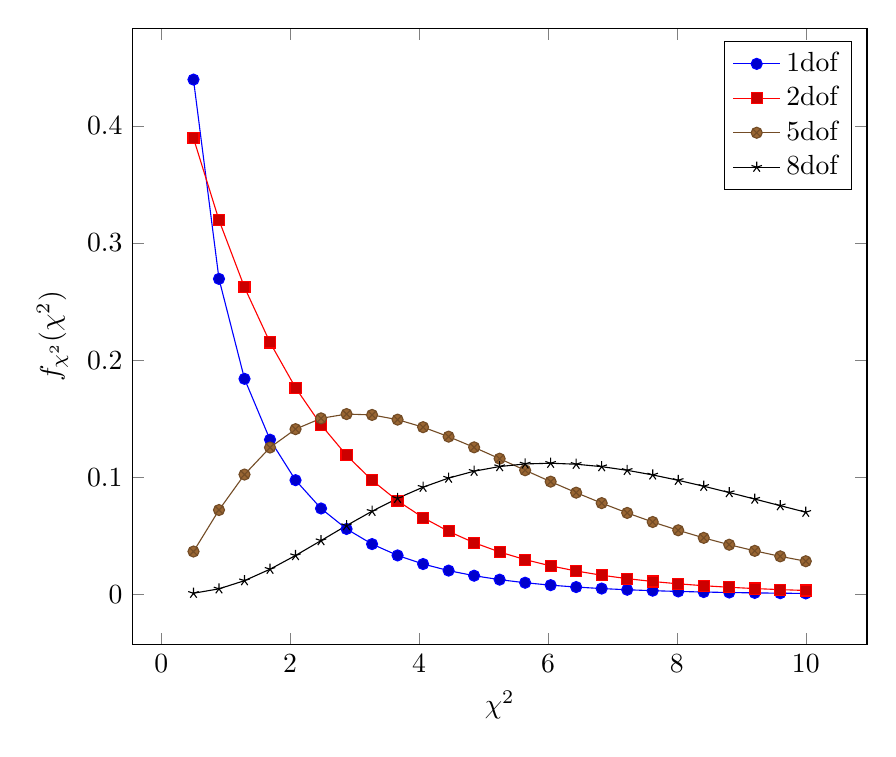
\begin{tikzpicture}
		\begin{axis}[
				width=.9\columnwidth,
				xlabel=$\chi^2$,
			ylabel=$f_{\chi^2}(\chi^2)$]
			\addplot+[domain={.5:10}] { exp( - .5 * x) / sqrt(2 * pi * x ) }; \addlegendentry{\SI{1}{\acs{dof}}}
			\addplot+[domain={.5:10}] { .5 * exp( - .5 * x ) }; \addlegendentry{\SI{2}{\acsp{dof}}}
			\addplot+[domain={.5:10}] { (x^(1.5)) * exp( - .5 * x )/ ( 3 * sqrt( 2 * pi ) ) }; \addlegendentry{\SI{5}{\acsp{dof}}}
			\addplot+[domain={.5:10}] { (x^(3)) * exp( - .5 * x )/ ( 96 ) }; \addlegendentry{\SI{8}{\acsp{dof}}}
		\end{axis}
	\end{tikzpicture}
	\caption{The $\chi^2$-distribution plot.}
	\label{fig:chi2distro}
\end{figure}
In figure~\ref{fig:chi2distro} is shown the plot of the $\chi^2$-distribution with only one \ac{dof}.
In this way
\begin{equation}
	P(\chi^2 > \chi^2_\textup{obs})
	= 
	\int_{\chi^2_\textup{obs}}^\infty f_{\chi^2}(\chi^2)\ud (\chi^2).
\end{equation}


\subsection{Generalization to two independent variables}

The joint \ac{pdf} is (no correlation terms appears because \acp{rv} are independent)
\begin{equation}
	f_x(x_1,x_2) = \frac{1}{2\pi\,\sigma_1\sigma_2}\exp\qp*{
		-\frac{(x_1-\mu_1)^2}{2\sigma_1^2}
		-\frac{(x_2-\mu_2)^2}{2\sigma_2^2}
	}.
\end{equation}
Now, define $\chi^2_i(x_i)\coloneqq (x_i-\mu_i)^2\!/\sigma_i^2$ for $i=1,2$ and hence the quantity $\chi^2(x_1,x_2) \coloneqq \chi^2_1(x_1) + \chi^2_2(x_2)$, which is a measure of the distance between the observed values $(x_1^\textup{obs},x_2^\textup{obs})$ and the means $(\mu_1,\mu_2)$.
Again, the equation $\chi^2 = \text{const.}$~defines contour lines in the $(x_1,x_2)$ planes which correspond to ellipses.


If the model is correct, what is the probability of obtaining measure result which corresponds to distances $\chi^2 > \chi^2_\textup{obs}$?
The answer is the integral of $f(x_1,x_2)$ over the region defined as the set $\Set{(x_1,x_2)\in\R^2|\chi^2 > \chi^2_\textup{obs}}$.
%\begin{equation}
%P( \chi^2 > \chi^2_\textup{obs} )  =
%\int_{\chi^2 > \chi^2_\textup{obs}}  f_{\chi^2}(\chi^2)\ud (\chi^2).
%\end{equation}•


\paragraph{Variables transformation}
Let's switch to using the $\chi^2$-variables from the $x$-variables using $f_{\chi^2}(\chi^2_1,\chi^2_2) = f_x(x_1,x_2)\,\abs{\det J}$.
Since each $\chi^2_i$ depends only on $x_i$, the partial derivatives become total derivatives and the Jacobian matrix is diagonal.


First let's switch to $(\chi_1,\chi_2)$ so
\begin{equation}\label{eq:chiIplane}
	f_{\chi_i}(\chi_1,\chi_2) = f_x(x_1,x_2)\,\abs{\det J} = f_x(x_1,x_2)\,\abs*{\deriv{\chi_1}{x_1}\,\deriv{\chi_2}{x_2}}^{-1} = \sigma_1\sigma_2 \frac{\eu^{-\chi^2_1/2 - \chi^2_2/2 }}{2\pi\,\sigma_1\sigma_2}.
\end{equation}
This distribution only depends on the radius $\chi^2  = \chi_1^2 + \chi_2^2$ hence $\chi^2 = \text{const.}$~defines circles in the $(\chi_1,\chi_2)$ space.


Let's express the~\eqref{eq:chiIplane} into polar coordinates $(\chi,\phi)$.
Since $\ud\chi_1\ud\chi_2 = \chi\ud\chi\ud\phi$ we have that
\begin{equation}
	f_\chi(\chi,\phi) = \frac{\chi\,\eu^{-\chi^2\!/2}}{2\pi}.
\end{equation}
As we already noticed, this is independent on the angle $\phi$ and therefore the marginalization is quite trivial:
\begin{equation}
	f_\chi(\chi) = \chi\,\eu^{-\chi^2\!/2}.
\end{equation}


In the last step we switch to $\chi^2$ as \ac{rv} using the fact that $2\chi\ud\chi = \ud(\chi^2)$ so
\begin{equation}
	f_{\chi^2}(\chi^2) = \frac{1}{2}\,\eu^{-\chi^2\!/2}.
\end{equation}
Now we can again evaluate
\begin{equation}
	P(\chi^2>\chi^2_\textup{obs}) = \int_{\chi^2_\textup{obs}}^\infty f_{\chi^2}(\chi^2)\ud(\chi^2).
\end{equation}

\subsection{Generalization to arbitrarily many \acsp{dof}}

Let's consider an array of $n$ independent \acp{rv} $\transpose{\vec{x}}\coloneqq(x_1,\dots,x_n)$.
\begin{equation}\label{eq:manyChi}
	f_x(\vec{x}) = \prod_{i=1}^n \frac{\eu^{-(x_i-\mu_i)^2\!/2\sigma_i^2}}{\sqrt{2\pi}\,\sigma_i}.
\end{equation}
Let's as before define $\chi^2_i(x_i) \coloneqq (x_i-\mu_i)^2\!/\sigma_i^2$ and $\chi^2 \coloneqq \chi^2_1+\dots+\chi^2_n$.
Now the equation $\chi^2\equiv\text{constant}$ will implicitly define hyper-ellipsoids in a $n$-dimensional euclidean space.


Switching to hyper-spherical coordinates the $\chi^2$-distribution~\eqref{eq:manyChi} reads
\begin{equation}\label{eq:manyChiSphere}
	f_{\chi^2}(\chi^2;n) = \frac{(\chi^2)^{(n-2)/2}\,\eu^{-\chi^2\!/2}}{2^{n/2}\,\Gamma(n/2)},
\end{equation}
where the number of independent \acp{dof} is indicated as a function parameter.


Now, for any value of $n$, the $\chi^2$ can be evaluated just by integrating over the upper tail distribution
\begin{equation}
	P(\chi^2>\chi^2_\textup{obs}) = \int_{\chi^2_\textup{obs}}^\infty f_{\chi^2}(\chi^2;n)\ud(\chi^2).
\end{equation}

\paragraph{Properties}
\begin{itemize}
	\item
		$E[\chi^2] = n$ i.e.~on average each data point (namely a \ac{dof}) contributes with one unit of $\chi^2$
	\item
		$V[\chi^2] = 2n$
	\item
		For large enough $n$, typically $n\gtrsim \num{40}$, the distribution $f_{\chi^2}$ tends to a Gau\ss{}ian one.
\end{itemize}

\Ex{%
	Suppose an absolute prediction for a distribution of some \ac{rv} $X$ is given, e.g.~a cross section---neglecting effects like efficiency, resolution, background and so on.
	We measure the number $n_i$ of events which lie in the $i$-th bin of $X$ and compare it with the predicted value $\mu_i$.
	If the prediction is correct, then $n_i$ should follow a Poisson distribution with mean $\mu_i$.
	For large enough $n_i$ the Poisson \ac{pdf} is well-approximated by a Gau\ss{}ian one with mean $\mu_i$ and variance $\mu_i$.

	Now we can utilize the $\chi^2$ statistic to check for consistency between data and prediction (i.e.~consistency of hypothesis).
	The $\chi^2$ reads
	\begin{equation}
		\chi_i^2 =\frac{(x_i -\mu_i)^2}{\mu_i},
	\end{equation}
	where in the denominator the \emph{expected} fluctuation from mean has been used.

	Let's consider $n=\num{20}$ and assume that the predicted \ac{pdf} is uniform $f(x)\equiv \num{500}$ for $x\in[0,1]$.
	So now we check the consistency of $n$ Gau\ss{}ian distributed \acp{rv} with the prediction by evaluating
	\begin{equation}
		\chi^2 = \sum_{i=1}^n \chi_i^2.
	\end{equation}
	If the hypothesis is correct, then $\chi^2$ should follow the~\eqref{eq:manyChiSphere} with $E[\chi^2] = \num{20}$ and $\sigma_{\chi^2} = \sqrt{\num{40}} \simeq \num{6.3}$.

	{\color{red} Copy plots}

	\begin{itemize}
		\item
			In the first case, we have $\chi^2_\textup{obs} = \num{16.2}$ with $P(\chi^2>\chi^2_\textup{obs}) \simeq \SI{70}{\percent}$: this is perfectly consistent with prediction;
		\item
			The second case, with $\chi^2_\textup{obs}=\num{41.5}$ and $P(\chi^2>\chi^2_\textup{obs}) = \SI{.3}{\percent}$, is a bit questionable;
		\item
			In the third case the agreement is ``too good to be real'' since $\chi^2_\textup{obs} = \num{3.3}\ll \num{20}$ and $P(\chi^2>\chi^2_\textup{obs}) = \SI{99.9992}{\percent}$.
			This looks like error bars have been overestimated since data-points fluctuation is too small compared to the uncertainties.

	\end{itemize}
}

\section{The $\chi^2$-fitting}

The $\chi^2$-fitting, or \ac{ls} method\index{least squares}, is a standard approach to approximate solution of overdetermined systems.
As its name suggest, the method consists in minimizing the sum of square \emph{residuals}\index{residual} i.e.~the $\chi^2$ function.\footnote{Residuals are defined as the difference between observed values and the one predicted by the model.}


This method is particularly useful for fitting of data since it determines the best estimate for parameters of model function.
Moreover it provides a \ac{gof} criterion.


Some assumptions have to be fulfilled:
\begin{itemize}
	\item
		The model has to describe data;
	\item
		Residuals have to be Gau\ss{}ian distributed.
\end{itemize}

\subsection{Combining measurements using \acs{ls}}

Let's consider a \ac{rv} $X$ with unknown true value $\mu$ measured $n$ times.
Thus we are dealing with $n$ independent values $\transpose{\vec{x} } \coloneqq (x_1,\dots,x_n)$ with uncorrelated Gau\ss{}ian uncertainties $\transpose{\vec{\sigma}} \coloneqq (\sigma_1,\dots,\sigma_n)$.


The \emph{residuals}\index{residuals} are defined as
\begin{equation}
	r_i \coloneqq x_i-\mu.
\end{equation}
We can weight them according to their uncertainties $\sigma_i$ and then minimize
\begin{equation}\label{eq:ChiSquareMuDummy}
	\chi^2(\mu) \coloneqq \sum_{i=1}^n \biggl(\frac{x_i - \mu}{\sigma_i}\biggr)^2
\end{equation}
with respect to its only argument $\mu$, since the $x_i$ are fixed.
Let $\hat \mu$ value of $\mu$ that minimizes the expression~\eqref{eq:ChiSquareMuDummy}, namely
\begin{equation}
	\deriv{}{\mu}\chi^2(\mu)\bigg\rvert_{\hat\mu} = 0 = -2\sum_{i=1}^n \frac{x_i-\hat\mu}{\sigma_i^2}.
\end{equation}
So the best estimate for the true value $\mu$ is
\begin{equation}
	\hat\mu = \frac{\sum_{i=1}^n x_i/\sigma_i^2}{\sum_{j=1}^n 1/\sigma_j^2}
\end{equation}
which is a \emph{weighted mean}\index{weighted!mean} i.e.~has the form
\begin{equation}
	\hat\mu = \sum_{i=1}^n w_ix_i
	\quad
	\text{with \emph{weights}\index{weight} }
	w_i \coloneqq \frac{1/\sigma_i^2}{\sum_{j}1/\sigma_j^2}.
\end{equation}

\paragraph{Variance of $\hat\mu$ from error propagation}

The best estimate $\hat\mu$ for the true value $\mu$ is itself a \ac{rv} and a function of $\vec{x}$ so
\begin{equation}
	V_{\hat\mu} = JV_X\transpose{J},
\end{equation}
where the Jacobian matrix is just a row matrix $J = \V \hat\mu = (w_1,\dots,w_n)$ and $V_X = \Set{\sigma_i^2\delta_{ij}}$ since the single $x_i$ measures are independent.
Thus
\begin{equation}
	V_{\hat\mu} = \sum_{i=1}^n w_i^2\sigma_i^2 = \frac{1}{\sum_j 1/\sigma_j^2}.
\end{equation}
\Ex{%
	Two values for a certain mass are measured $(x_1,x_2) = (\num{5.1},\num{6.0})$ with uncertainties $(\sigma_1,\sigma_2) = (\num{.5},\num{.3})$.
	The best estimate for the mean is then $\hat\mu = \num{5.76 +- .26}$.
}


\paragraph{Variance of $\hat\mu$ via Taylor expansion}
Let's expand $\chi^2(\mu)$ around its minimum $\hat\mu$ using the fact that $\ud\chi^2(\hat\mu)/\!\ud\mu = 0$ and all derivatives with order greater than two vanish:
\begin{equation}
	\chi^2(\mu) = \chi^2(\hat\mu) +\frac{1}{2} \deriv[2]{}{\mu}\chi^2\bigg\rvert_{\hat\mu}(\mu-\hat\mu)^2.
\end{equation}\label{eq:chiSquareExpansion}
Substituting this expression in the joint \ac{pdf}~\eqref{eq:manyChi} one has
\begin{equation}
	f_{\chi^2} \propto \eu^{-\chi^2_{\textup{min}}/2}\exp\biggl\{ -\frac{1}{2} \biggl[\frac{1}{2} \deriv[2]{}{\mu}\chi^2\bigg\rvert_{\hat\mu}(\mu-\hat\mu)^2\biggr]\biggr\},
\end{equation}
which is again a Gau\ss{}ian in $\mu$ with variance
\begin{equation}
	\sigma^2_{\hat\mu} = \frac{1}{\dfrac{1}{2} \deriv[2]{}{\mu}\chi^2\bigg\rvert_{\hat\mu}} = \frac{1}{\sum_j 1/\sigma_j^2}   = V_{\hat\mu}.
\end{equation}
Both approaches are equivalent!


Now an important result comes out.
\begin{figure}
	\centering
	\begin{tikzpicture}
		\begin{axis}[
				samples=50,
				%     title={Test Axis},
				axis x line=middle,
				axis y line=middle,
				xtick={1,2,3},
				xticklabels={{$\hat\mu-\sigma_{\hat\mu}$},{$\hat\mu$},{$\hat\mu+\sigma_{\hat\mu}$}},
				ytick={0,1,2},
				yticklabels={{$0$},{$\chi^2_\textup{min}$},{$\chi^2_\textup{min}$+1}},
				xlabel={$\mu$},
				ylabel={$\chi^2(\mu)$},
				%	enlargelimits=.05,
			]
			\addplot+[
				%name path global=one,
				domain={-.1:4.1},%
				mark=none%
			] {(x-2)^2 + 1 };

			%	\addplot [name path global=two, red, domain={.5:3.5},opacity=.4] {2};
			%	\path [draw,name intersections={of=one and two, by={A,B}}];

			% to force axis in the origin
			\addplot [ red, domain={.5:3.5},opacity=.0] {0};


			%	\addplot [name path global=three, black, domain={0:2}, dashed,opacity=.4] {1};
			%	\path [draw,name intersections={of=one and three, by={C}}];

		\end{axis}

		% draw projections
		\coordinate (O); % set (O)=(0,0)
		%\foreach \p in {A,B} {
		%	\path[draw=black, dashed] (\p) -- (\p|-O);
		%}
		%	\path[draw=black,dashed,opacity=.4] (C) -- (C|-O);

	\end{tikzpicture}
	\caption{Plot of $\chi^2(\mu)$ with contour line at $\chi^2_\textup{min} + 1$.}
	\label{fig:chiSquareIntervalStuff}

\end{figure}
By substituting the expression for the variance on $\hat\mu$ into the expansion~\eqref{eq:chiSquareExpansion} one sees that
\begin{equation}
	\chi^2(\hat\mu\pm\sigma_{\hat{\mu}} ) = \chi^2(\hat\mu) + \frac{(\hat\mu\pm\sigma_{\hat\mu}-\hat\mu)^2}{\sigma_{\hat\mu}^2} = \chi^2_\textup{min} + 1.
\end{equation}
As it's shown in figure~\ref{fig:chiSquareIntervalStuff}, the value of $\mu$ such that $\chi^2(\mu) = \chi^2_{\textup{min}} + 1$ is \emph{always} \SI{1}{\ensuremath{\sigma_{\hat\mu}}} far away from $\hat\mu$.


\Ex{%
	Given a set of measures $\Set{x_i\pm\sigma_i}_{i=1}^N$, one has that $\sigma_{\hat\mu} < \sigma_i$ for each $i = \Set{1,\dots,N}$.
	Moreover, if there is one index $j$ such that $\sigma_j \ll \sigma_i$ for each $i\neq j$, then this measure will dominate mean and variance.
}

\subsection{Generalization to correlated measurements}

The joint \ac{pdf} for $N$ Gau\ss{}ian-distributed correlated measurements is
\begin{equation}
	f_x(\vec{x}) = \frac{\eu^{-\transpose{(\vec{x}-\vec{\mu})}V^{-1}(\vec{x}-\vec{\mu})/2}}{\sqrt{(2\pi)^n\det V}}
\end{equation}
where $\vec{\mu} = (\mu,\dots,\mu)$.
We define
\begin{equation}
	\chi^2(\mu) \coloneqq \transpose{(\vec{x}-\vec{\mu})}V^{-1}(\vec{x}-\vec{\mu})
\end{equation}
so now we can impose that the first derivative with respect to $\mu$ vanishes to obtain
\begin{equation}
	\hat\mu = 
	\frac{\sum_{i,j}(V^{-1})_{ij}x_j}{\sum_{i,j}(V^{-1})_{ij}}.
\end{equation}
Again, one can derive the variance from the error propagation or using
\begin{equation}
	\sigma^2_{\hat\mu} = \frac{1}{\dfrac{1}{2} \deriv[2]{}{\mu}\chi^2\bigg\rvert_{\hat\mu}} = \frac{1}{\sum_{i,j} (V^{-1})_{ij}}   = V_{\hat\mu}.
\end{equation}

\Th[Gau\ss{}-Markov]{%
	$\hat\mu\pm\sigma_{\hat\mu}$ is a zero-bias estimate with minimum variance.
}


\section{Fitting function parameters using \acs{ls} method}

Fitting functions parameters is the most important application of the \ac{ls} method.
To achieve it, a change of notation is needed.


A set of $n$ data $\Set{y_i\pm\sigma_i}_{i=1}^n$ is given.
The goal is to find the best estimate for unknown parameters $\transpose{\vec{\theta}} \coloneqq (\theta_1,\dots,\theta_m)$ of the model function $y = f(x;\vec{\theta})$ that describes data.


As an assumption, the $y_i$ are independent, Gau\ss{}ian-distributed \acp{rv} and for every value of $x$, the model function $y=f(x;\vec{\theta})$ predicts the $y$ value.


The array of means is given by $\vec{f}(\vec{\theta}) \coloneqq (f(x_1;\vec{\theta}),\dots,f(x_n;\vec{\theta}))$ with uncorrelated uncertainties $\vec{\sigma}\coloneqq (\sigma_1,\dots,\sigma_n)$.
The values of $\vec{x}\coloneqq (x_1,\dots,x_n)$ which correspond to $\vec{y}$ are assumed to be known exactly.


The joint \ac{pdf} for \vec{y} is
\begin{equation}
	\begin{aligned}
		f_{y}(\vec{y}) &= \prod_{i=1}^n \frac{1}{\sqrt{2\pi}\,\sigma_i}
		\exp\qp[\bigg]{%
			-\frac{1}{2} \tp[\bigg]{%
				\frac{y_i - f(x_i;\vec{\theta})}{\sigma_i}
			}^2
		}\\
		&=
		\tp[\bigg]{%
			\prod_{i=1}^n
			\frac{1}{\sqrt{2\pi}\,\sigma_i}
		}
		\exp\qp[\bigg]{%
			-\frac{1}{2} \sum_{i=1}^n\chi^2_i(\vec{\theta})
		}.
	\end{aligned}
\end{equation}
The best estimate for \vec{\theta} is obtained by minimizing
\begin{equation}
	\chi^2(\vec{\theta}) \coloneqq\sum_{i=1}^n\chi^2_i(\vec{\theta}).
\end{equation}
This will lead to solving $m$ normal equations (recall $m$ is the number of free parameters) of the form
\begin{equation}\label{eq:NormEqs}
	0 = \pderiv{\chi^2}{\theta_j}\bigg\rvert_{\vec{\theta}=\hat{\vec{\theta}}}
	=
	-2
	\sum_{i=1}^n \frac{y_i - f(x_i;\vec{\theta})}{\sigma_i^2}\,\pderiv{}{\theta_j}f(x_i;\vec{\theta})\bigg\rvert_{\vec{\theta} =\hat{\vec{\theta}}},
	\qquad
	\forall j\in\Set{1,\dots,m}.
\end{equation}


Now we need to specialize: the form of the model function $f(x;\vec{\theta})$ determines the method to work out the solution.

\paragraph{Linear case}
The model is linear in the parameters $\theta_i$ i.e.~it has the form
\begin{equation}
	f(x;\vec{\theta}) = \sum_{i=1}^m \theta_ia_i(x),
\end{equation}
where $\Set{a_i(x)}_{i=1}^m$ is a set of linearly independent functions.
In this case, the normal equations~\eqref{eq:NormEqs} can be solved in a closed form.


\Ex{%
	The function $f(x;\vec{\theta}) = \theta_1 +\theta_2x+\theta_3 \sqrt{x} + \theta_4\ln x$ is linear in the parameters whereas $g(x;\vec{\theta}) = \theta_1 + \sin(x+\theta_2)$ is not, even though it looks easier.
	A possible approach for $g$ could be a Taylor expansion at first order in $\theta_2$ provided that there is some reason to assume the parameter is small enough.
}

\paragraph{Non-linear case}
The model function is \emph{not} linear in its parameters $\vec{\theta}$.
Sometimes it's possible to linearize the function and step back to the previous case but, in general, a solution can be obtained only by numerical methods.

\subsection{\acs{ls} method for linear model functions}

In what follows, only the linear case will be considered.
We'll allow correlated measures so that
\begin{equation}
	f_y (\vec{y}) = \frac{1}{\sqrt{(2\pi)^n\det V}}\exp
	\qp[\bigg]{%
		-\frac{1}{2}\transpose{(\vec{y} - \vec{f}(\vec{\theta}))}V_y^{-1}(\vec{y} - \vec{f}(\vec{\theta}))
	}.
\end{equation}
Since $f$ is linear in its parameters, we can define the matrix
\begin{equation}\label{eq:linearMatDefinition}
	f(x_i;\vec{\theta}) = \sum_{j=1}^m \theta_ja_j(x_i) \eqqcolon (A\vec{\theta})_i,
\end{equation}
where $A = \Set{A_{ij}} \coloneqq \Set{a_j(x_i)}$ is an $(n\x m)$-matrix.
Moreover, from equation~\eqref{eq:linearMatDefinition} one can derive
\begin{equation}
	A_{ij} = \pderiv{}{\theta_j}f(x;\vec{\theta})\bigg\rvert_{%x=
	x_i}.
\end{equation}
The $\chi^2$ now reads
\begin{equation}\label{eq:ChiSquareFunctionLinear}
	\chi^2(\vec{\theta}) = \transpose{(\vec{y} - A\vec{\theta})}V_y^{-1}(\vec{y} - A\vec{\theta}).
\end{equation}
The best estimate for the parameters will be such that
\begin{equation}
	\V \chi^2\rvert_{\hat{\vec{\theta}}} = 0.
\end{equation}


Recall from the matrix calculus that
\begin{equation}
	\pderiv{\transpose{\vec{x}}\vec{y}}{\vec{x}} = 
	\pderiv{\transpose{\vec{y}}\vec{x}}{\vec{x}} = \vec{y}
\end{equation}
and that for a symmetric matrix
\begin{equation}
	\pderiv{\transpose{\vec{x}}S\vec{x}}{\vec{x}} = 2S\vec{x}.
\end{equation}
In these formulas, neither \vec{y} nor $A$ depend on $\vec{x}$.


Hence
\begin{equation}
	\begin{aligned}
		\chi^2(\vec{\theta})
		&= \transpose{(\vec{y} - A\vec{\theta})}(V_y^{-1}\vec{y} -V_y^{-1}A\vec{\theta}) \\
  &= \transpose{\vec{y}}V_y^{-1}\vec{y} - \transpose{\vec{\theta}}\transpose{A}V_y^{-1}\vec{y}
		-\transpose{\vec{y}}V_y^{-1}A\vec{\theta} + \transpose{\vec{\theta}}\transpose{A} V_y^{-1} A\vec{\theta}
	\end{aligned}
\end{equation}
Now we'll use the fact that $V_y^{-1}$ is symmetric so $\transpose{(V_y^{-1})}=V_y^{-1}$ and the properties of the scalar product $\transpose{\vec{y}}V_y^{-1}A\vec{\theta} = \transpose{\vec{\theta}}\transpose{A}V_y^{-1}\vec{y}$.
So evaluating the derivative with respect to the free parameters
\begin{equation}
	0 = \V \chi^2(\vec{\theta})\rvert_{\hat{\vec{\theta}}} = -2 \transpose{A}V_y^{-1} \vec{y} + 2 (\transpose{A}V_y^{-1}A)\hat{\vec{\theta}},
\end{equation}
where it's worth noting that $\transpose{A}V_y^{-1}A$ is a symmetric $(m\x m)$-matrix.
From here it's easy to see that, assuming that $\transpose{A}V_y^{-1}A$ is invertible,
\begin{equation}
	\hat{\vec{\theta}} = (\transpose{A}V_y^{-1}A)^{-1} \transpose{A}V_y^{-1}\vec{y}
	\eqqcolon B\vec{y}
\end{equation}
is the best estimator for the function parameters.
We get that the parameters $\hat{\vec{\theta}}$ are a \emph{linear} function of collected data $\vec{y}$ and $B$ is a $(m\x n)$-matrix.


The uncertainties for the parameters can be evaluated using the error propagation $V_{\hat{\theta}} = J V_y\transpose{J}$.
The components of the Jacobian matrix are
\begin{equation}
	J_{ij} = \pderiv{\hat{\theta}_i}{y_j} = B_{ij},
\end{equation}
thus we have that $J=B$ and
\begin{equation}
	\begin{aligned}
		V_{\hat{\theta}}
		&= B V_y\transpose{B}\\
  &= (\transpose{A}V_y^{-1}A)^{-1} \transpose{A}V_y^{-1}V_y\transpose{[(\transpose{A}V_y^{-1}A)^{-1} \transpose{A}V_y^{-1}]}\\
  &= (\transpose{A}V_y^{-1}A)^{-1} (\transpose{A}V_y^{-1}A) (\transpose{A}V_y^{-1}A)^{-1} \\
  &= (\transpose{A}V_y^{-1}A)^{-1}.
	\end{aligned}
\end{equation}


From equation~\eqref{eq:ChiSquareFunctionLinear}, where the linearity property of the function $f(x_i;\vec{\theta}) = A \vec{\theta}$ has already been used, one can see that $\chi^2$ is quadratic in the parameters $\vec{\theta}$ so that the second-order expansion
\begin{equation}
	\chi^2(\vec{\theta}) = 
	\chi^2(\hat{\vec{\theta}}) + \frac{1}{2}\sum_{i,j=1}^m \pderiv{^2\chi^2}{\theta_i\de\theta_j}\bigg\rvert_{\hat{\vec{\theta}}} (\theta_i - \hat\theta_i) (\theta_j - \hat\theta_j)
\end{equation}
holds \emph{exactly}.
Here the first order derivative vanishes in $\hat{\vec{\theta}}$ and derivatives of order greater than two vanish as well.
Substituting the expansion in the joint \ac{pdf} for $\vec{y}$
\begin{equation}
	f_y(\vec{y}) \propto \eu^{\transpose{(\vec{\theta} - \hat{\vec{\theta}})} W (\vec{\theta} - \hat{\vec{\theta}})/2},
\end{equation}
we see that $W = V_{\hat\theta}^{-1}$ so
\begin{equation}
	W_{ij} =  \frac{1}{2}\pderiv{^2\chi^2}{\theta_i\de\theta_j}\bigg\rvert_{\hat{\vec{\theta}}} = (V_{\hat\theta}^{-1})_{ij}.
\end{equation}
Again the equation $\chi^2(\vec{\theta}) = \chi^2(\hat{\vec{\theta}}) + 1$ implicitly defines a contour which corresponds to intervals $\hat\theta_i \pm \sigma_{\hat{\theta}_i}$, i.e.~to one \ac{sd} deviation departures from the best \ac{ls} estimates.
In this case, the contours are hyperellipsoids.



In the non-linear case the $\chi^2(\vec{\theta})$ function can be approximated by a Taylor expansion around its minimum $\chi^2_\textup{min}$ up to the second order.
This will lead to an approximate value for the uncertainties $V_{\hat\theta}$.
However in this case the contour lines defined by $\chi^2(\vec{\theta}) = \chi^2_\textup{min} + 1$ will \emph{not} be elliptical anymore.


In both cases the volume of the region enclosed in the contour line defined by the equation $\chi^2(\vec{\theta}) = \chi^2_\textup{min} + 1$ reflects the statistical uncertainty of the fitted parameters.
\begin{table}
	\centering
	\caption{Probabilities (i.e.~confidence levels) of the \SI{1}{\ensuremath{\sigma}} region for different numbers of parameters $m$.}
	\label{tab:ConfLevelLSestimate}
	\begin{tabular}{>$r<$ S}
		\toprule
		m &{\ensuremath{P} (\si{\percent})}\\
		\midrule
		1 	&68.3\\
		2	&39.4\\
		3	&19.9\\
		\bottomrule
	\end{tabular}
\end{table}
As the table~\ref{tab:ConfLevelLSestimate} shows, this volume depends on the number of free parameters $m$.

\section{\acl{gof}}

In the derivation of the \ac{ls} method we assumed that the model described data.
Now we are left with the question <<does the model describe data?>>
Here is clear that \ac{gof} and parameter estimation are indeed \emph{logically separate} things.
%However the advantage of the \ac{ls} method is that it automatically gives 

\subsection{\acl{gof} with $\chi^2$}

Let's start by remarking that the $\chi^2$-statistics is a ``number which is calculated from the data'' and it's \emph{different} from the $\chi^2$-\ac{pdf}.
The $\chi^2$-statistic is a \ac{rv} itself and is, as a function of the parameters,
\begin{equation}
	\chi^2(\vec{\theta}) = \transpose{(\vec{y} - \vec{f}(\vec{\theta}))}V_y^{-1}(\vec{y} - \vec{f}(\vec{\theta})).
\end{equation}
Thus, $\chi^2_\textup{min}$ is a measure for the total  agreement of model with data when:
\begin{enumerate}[(i)]
	\item
		The \ac{rv} $Y$ is Gau\ss{}ian-distributed with known variance matrix $V_y$;
	\item
		The model function $\vec{f}(x;\vec{\theta})$ is linear in the parameters $\vec{\theta}$;
	\item
		The model actually describes data.
\end{enumerate}
Under these conditions $\chi^2_\textup{min}$ is also distributed according to a $\chi^2$-\ac{pdf} with a number of \ac{dof} equal to $n-m\eqqcolon d$.
Since $E[\chi^2] = d$ we can define the reduced $\chi^2$ as
\begin{equation}
	\chi^2_\textup{red} \coloneqq \frac{\chi^2_\textup{min}}{d}.
\end{equation}
There are again three cases:
\begin{itemize}
	\item
		If $\chi^2_\textup{red} \simeq 1$ then everything is as expected and everybody is happy.
	\item
		If $\chi^2_\textup{red} \ll 1$ then the fit is better than expected.
		In this case there is no evidence against the model function (unless one is in over-fitting regime) but it can be due to overestimated errors or good luck---as a last resort.
	\item
		If $\chi^2_\textup{red} \gg 1$ then the fit is worse than expected.
		This may depend on several reasons: first of all it could be a reason to doubt about some of the model hypothesis.
		Anyway, it could also be due  to underestimated errors as well as bad measurements.
		As a last resort, again, one could just claim it's bad luck.
\end{itemize}



The \emph{significance level}\index{significance level} is given by $P(\chi^2 > \chi^2_\textup{obs})$ e.g.~if $P(\chi^2 > \chi^2_\textup{obs}) = \num{.2}$ it means that, provided that the true function is the model function, after repeating the experiment many times in \SI{20}{\percent} of cases the value of the $\chi^2$ will be greater than $\chi^2_\textup{obs}$.
A test based on the $P$-value can only reject hypothesis after defining a certain threshold which, in principle, is arbitrary.
A common choice is to fix this value to \SI{1}{\percent} or \SI{5}{\percent}.



The $P$-value is heavily based on the knowledge of the matrix $V_y$ therefore underestimated errors or uncorrecr treatment of correlations can cause large $\chi^2$.
\begin{figure}
	\centering
	\color{red}
	plot figures
	\caption{Two data sets with different $y_i$ but same $\sigma_i$ are shown. They've got the same weighted mean \num{.38\pm.05} i.e.~the $\chi^2$ parabola is simply shifted with the same curvature.}
	\label{fig:ChiSquareMindBlow}
\end{figure}
It's also worth noting that, as the figure~\ref{fig:ChiSquareMindBlow} shows, a small value for the $\chi^2_\textup{min}$ \emph{does not mean} that the parameters have been estimated with small uncertainties.
In fact $V_{\hat{\theta}} = (\transpose{A}V_u^{-1}A)^{-1}$, where $A_{ij} = a_j(x_i)$, is \emph{independent} on the measured $y_k$.
The statistical uncertainties are given by the change of $\chi^2$ when the parameters are moved from the best estimates so they don't depend on $\chi^2_\textup{min}$.


The value of the $\sigma_{\hat\theta_i}$ for the estimator $\hat\theta_i$ is a measure of how widely the estimator would spread if the experiment is repeated many times.
If the model function \emph{does not} describe the data, $\hat\theta_i$ might be significantly different from the true value!
Therefore a small $\sigma_{\hat\theta_i}$ is not sufficient to infer that the uncertainty on the parameter $\theta_i$ is small.



The \ac{gof} tells whether data are consistent {\color{red}with having been drown} from specific distribution: it compares the model to all the possible ways a random data might fluctuate.
On the other hand, the parameter estimation finds which, out of a set of hypothesis, is the most consistent with data.

\begin{figure}
	\color{red}figure
\end{figure}
%For instance, in the figure~\ref{fig:ChiSquareDIfferentGoF}


As the number $d$ of \acp{dof} grows the \ac{pdf} for $\chi^2_\textup{red}$ becomes closer and closer to a Gau\ss{}ian distribution centered around \num{1}.
\begin{figure}
	\centering
	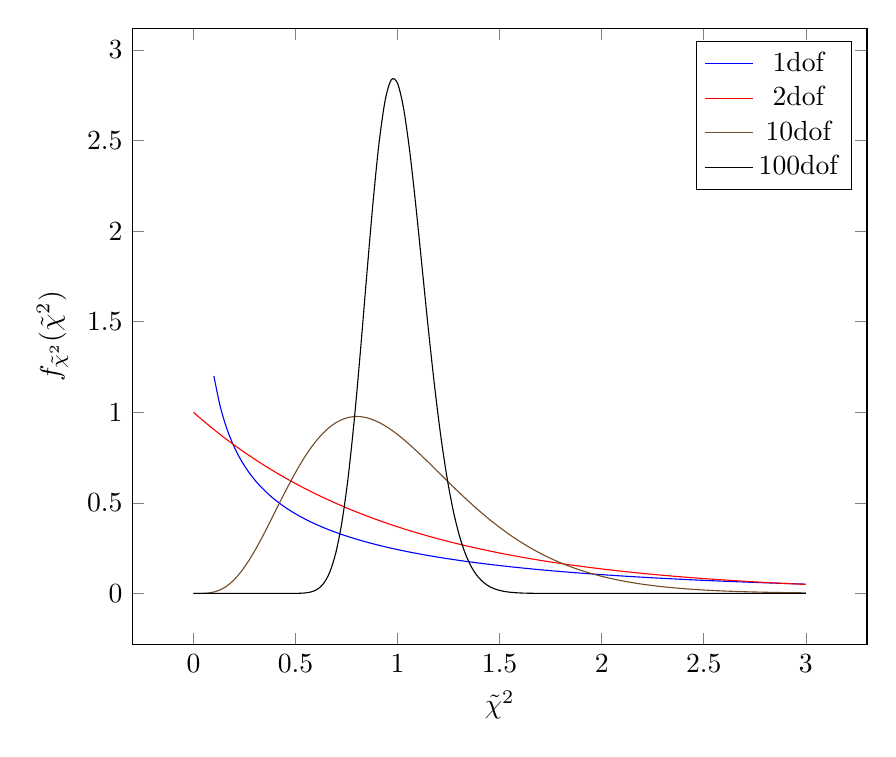
\begin{tikzpicture}
		\begin{axis}[
				width=.9\columnwidth,
				xlabel=$\tilde\chi^2$,
				ylabel=$f_{\tilde\chi^2}(\tilde\chi^2)$,
				samples=100,
				smooth
			]
			\addplot+[domain={.1:3},mark=none] { exp( - .5 * x) / sqrt(2 * pi * x ) }; \addlegendentry{\SI{1}{\acs{dof}}}
			\addplot+[domain={0:3},mark=none] { exp( - x ) }; \addlegendentry{\SI{2}{\acsp{dof}}}
			%	\addplot+[domain={0:3}] { 7.4338504839698796 * (x^(1.5)) * exp( - 2.5 * x )) }; \addlegendentry{\SI{5}{\acsp{dof}}}
			\addplot+[domain={0:3},mark=none] { 130.20833333333 * (x^(4)) * exp( - 5 * x ) }; \addlegendentry{\SI{10}{\acsp{dof}}}
			\addplot+[domain={0:3},mark=none] { 1.46014285845959 * (10^22) * (x^(49)) * exp( - 50 * x ) }; \addlegendentry{\SI{100}{\acsp{dof}}}
		\end{axis}
	\end{tikzpicture}
	\caption{The $\tilde\chi^2$-distribution plot with different number of \acp{dof}.}
	\label{fig:RedChiSquareDistro}
\end{figure}
Using the general expression for $f_{\chi^2}(\chi^2;n)$ given in equation~\eqref{eq:manyChiSphere} and the fact that $\ud\tilde\chi^2=\ud(\chi^2\!/n) = (\ud\chi^2)/n$ it's easy to derive the \ac{pdf} for the reduced $\chi^2$
\begin{equation}
	f_{\tilde\chi^2}(\tilde\chi^2;n) = \biggl(\frac{n\tilde\chi^2}{2}\biggr)^{n/2} \frac{\eu^{-n\tilde\chi^2\!/2}}{\tilde\chi^2\Gamma(n/2)}.
\end{equation}
Figure~\ref{fig:RedChiSquareDistro} shows the plot of $f_{\tilde\chi^2}$ for some value of the number of \acp{dof}.
As $n$ grows, the distribution becomes more and more peaked around \num{1} so the values of $\chi^2\!/n$ which correspond to the same significance level move closer to \num{1} with increasing number of \acp{dof}.
\begin{equation}\label{eq:ProbChiSquareGeneral}
	%\begin{aligned}
	P(\tilde\chi^2>\tilde\chi^2_\textup{obs}) 
	%= \int_{\tilde\chi^2_\textup{obs}}^\infty f_{\tilde\chi^2}(\tilde\chi^2;n)\ud(\tilde\chi^2)%\\
	=\int_{\tilde\chi^2_\textup{obs}}^\infty \biggl(\frac{n\tilde\chi^2}{2}\biggr)^{n/2} \frac{\eu^{-n\tilde\chi^2\!/2}}{\tilde\chi^2\Gamma(n/2)}\ud(\tilde\chi^2)%\\
	= \int_{n\tilde\chi^2_\textup{obs}/2}^\infty \frac{x^{(n-2)/2}\eu^{-x}\ud x}{\Gamma(n/2)}.
\end{equation}
Now we'll assume $n$ is even and greater than or equal to \num{2} so that $n/2-1$ is integer and greater than or equal to \num{0}.
Under these hypothesis the integral can be written as
\begin{equation*}
	P(\tilde\chi^2>\tilde\chi^2_\textup{obs})  =
	\abs*{\deriv[n/2-1]{}{\alpha}\int_{x_\textup{obs}}^\infty\frac{\eu^{-\alpha x} \!\ud x}{\Gamma(n/2)}}_{\alpha=1}
	= \frac{1}{\Gamma(n/2)}\abs*{\deriv[n/2-1]{}{\alpha}\frac{\eu^{-\alpha x_\textup{obs}}}{\alpha}}_{\alpha=1},
\end{equation*}
where the parameter $\alpha$ is assumed to be positive and $x_\textup{obs} \coloneqq n\tilde \chi^2_\textup{obs}/2$.
Hence
\begin{equation*}
	\begin{aligned}
		P(\tilde\chi^2>\tilde\chi^2_\textup{obs})
		&= \frac{1}{\Gamma(n/2)}
		\abs*{\sum_{k=0}^{n/2-1}{n/2-1 \choose k}
			\tp*{\deriv[n/2-(k+1)]{}{\alpha}\eu^{-\alpha x_\textup{obs}}}
			\tp*{\deriv[k]{}{\alpha}\frac{1}{\alpha}}
		}_{\alpha=1}\\
		&= \frac{1}{\Gamma(n/2)}
		\abs*{\sum_{k=0}^{n/2-1}{n/2-1 \choose k}
			%\tp*{\frac{\chi^2_\textup{obs}}{2}}
			x_\textup{obs}^{n/2-(k+1)}\eu^{-\alpha x_\textup{obs}}
			\frac{(-1)^kk!}{\alpha^{k+1}}
		}_{\alpha=1}\\
		&= \frac{1}{\Gamma(n/2)}
		\abs*{\sum_{k=0}^{n/2-1}\frac{(n/2-1)!}{ (n/2 - (k+1))!}
			%\tp*{\frac{\chi^2_\textup{obs}}{2}}
			x_\textup{obs}^{n/2-(k+1)}
			(-1)^k
		}\\
		&=
		\abs*{
			\sum_{k=0}^{n/2-1}\frac{(-1)^kx_\textup{obs}^{n/2-(k+1)}}{(n/2 - (k+1))!}
			%\tp*{\frac{\chi^2_\textup{obs}}{2}}
		}.
	\end{aligned}
\end{equation*}
It's convenient to change the index introducing $m\coloneqq n/2-(k+1)$, which will run from $n/2-1$ to $0$.
The index $m$ can again be renamed after $k$ so, plugging in back the value for $x_\textup{obs}$, we get
\begin{equation}
	P(\tilde\chi^2>\tilde\chi^2_\textup{obs})
	=
	\abs*{(-1)^{n/2-1}
		\sum_{k=0}^{n/2-1}\frac{(-1)^k}{k!}
		\tp*{\frac{\chi^2_\textup{obs}}{2}}^{k}
	}
	=
	\sum_{k=0}^{n/2-1}\frac{n^k}{k!}
	\tp*{-\frac{\tilde \chi^2_\textup{obs}}{2}}^{k}.
\end{equation}
If $\tilde\chi^2_\textup{obs} = 0$ then we recover the proper normalization, i.e.~$P(\tilde\chi^2 > 0) = 1$.
When $n\to\infty$ (recall that $n$ is even) the result is
\begin{equation}
	\lim_{n\to\infty}P(\tilde\chi^2>\tilde\chi^2_\textup{obs}) = \eu^{-\chi^2_\textup{obs}/2},
\end{equation}
which is no longer a function of $n$.


When $n$ is odd, one can again start from the general formula~\eqref{eq:ProbChiSquareGeneral}.
Defining, as before, $x_\textup{obs} \coloneqq n\tilde\chi^2_\textup{obs}/2$ and writing $m -1/2\coloneqq n/2-1$ such that now $m$ is a natural number and if $n=1$ then $m=0$ one can see that (recall $\Gamma(n/2) = \Gamma(m+1/2)$)
\begin{equation}
	P(\tilde\chi^2>\tilde\chi^2_\textup{obs}) = \frac{f(m,x_\textup{obs})}{\Gamma(m+1/2)}.
\end{equation}
This function is such that $f(m,0) = 1$ and $\lim_{x_\textup{obs}\to\infty}f(m,x_\textup{obs}) = 0$.
Now we'll find a recursive formula for $f(m,x_\textup{obs})$
\begin{equation}
	\begin{aligned}
		f(m;x_\textup{obs})
		&=  \int_{x_\textup{obs}}^\infty x^{m-1/2}\eu^{-x}\!\ud x\\
  &= -x^{m-1/2}\eu^{-x}\big\rvert_{x_\textup{obs}}^\infty - \biggl(m-\frac{1}{2}\biggr) \int_{x_\textup{obs}}^\infty x^{(m-1)-1/2}\eu^{-x}\!\ud x\\
  &= x_\textup{obs}^{m-1/2}\eu^{-x_\textup{obs}}- \biggl(m-\frac{1}{2}\biggr) f(m-1,x_\textup{obs}).
	\end{aligned}
\end{equation}
Now we note that
\begin{equation}
	\begin{aligned}
		f(0;x_\textup{obs})
		&=  \int_{x_\textup{obs}}^\infty \frac{\eu^{-x}}{\sqrt{x}}\ud x
		=  \int_{\sqrt{x_\textup{obs}}}^\infty \eu^{-y^2}\!\ud y
		= \frac{1}{2}\biggl(\int_\R - \int_{\sqrt{x_\textup{obs}}}^{\sqrt{x_\textup{obs}}}\biggr) \eu^{-y^2}\!\ud y\\
		&= \frac{\sqrt{\pi}}{2} - \int_0^{\sqrt{x_\textup{obs}}}\eu^{-y^2}\!\ud y
		=  \frac{\sqrt{\pi}}{2}(1-\erf(\sqrt{x_\textup{obs}}))
	\end{aligned}
\end{equation}

[TODO: finish this]


The distribution of $P(\chi^2 > \chi^2_\textup{obs})$ is uniform if the model describes data \emph{and} the errors are distributed according to a Gau\ss{}ian.
\begin{figure}
	\centering
	\begin{tikzpicture}
		\begin{axis}[
				xlabel = {$P(\tilde\chi^2>\tilde\chi^2_\textup{obs})$},
				ylabel = {Relative frequency}
			]
			\addplot+ [mark=none] table {probChiSquareLaplace.dat};\label{curve:laplace}\addlegendentry{Laplace}
			\addplot+ [mark=none] table {probChiSquareGauss.dat};\addlegendentry{Gau\ss{}}
			%\addplot[domain=0:240] {70.1}
		\end{axis}
	\end{tikzpicture}
	\caption{Data errors for the blue curve (\ref{curve:laplace}) are distributed according to a Laplacian distribution~\eqref{eq:laplacianDistribution}.}
	\label{fig:chiSquareProbNonFlat}
\end{figure}
In real-life experiments it happens that
\begin{enumerate}[i.]
	\item
		Data are a mixture of signal and background processes;
	\item
		Measures are not distributed according to a Gau\ss{}ian.
\end{enumerate}
For these reasons, the $\chi^2$-probability distribution often looks like the one shown in figure~\ref{fig:chiSquareProbNonFlat} with peaks in correspondence of the values \num{0} and \num{1}.
In the figure the model indeed described data but errors where generated according to a Laplacian distribution
\begin{equation}\label{eq:laplacianDistribution}
	L(x;\mu,b) \coloneqq \frac{\eu^{-\abs{x-\mu}/b}}{2b}.
\end{equation}



In general the $\chi^2$-probability distribution will look like the one plotted in figure~\ref{fig:chiSquareProbNonFlat} where
\begin{itemize}
	\item
		The first peak in $P = 0$ corresponds to $\tilde\chi^2\gg1$.
		This may be due to
		\begin{enumerate}[i)]
			\item
				Background processes which are not described by the model;
			\item
				Bad fit (i.e.~not converged, pathological solutions\dots);
			\item
				Subset with underestimated uncertainties.
		\end{enumerate}
	\item
		The second peak in $P=1$, corresponding to $\tilde\chi^2\ll1$, may be due to
		\begin{enumerate}[i)]
			\item
				Subset with overestimated errors;
			\item
				Processes where the model function has too many parameters, thus leading the fit process into \emph{over-fitting} regime;
		\end{enumerate}
\end{itemize}



Never rely only on $\chi^2_\textup{min}$: always perform a \ac{gof} check ``by eye''.
\begin{itemize}
	\item
		The plot of residuals\index{residual} $r_i \coloneqq y_i - f(x_i;\vec{\hat\theta})$ should be consistent with the zero-line;
	\item
		The plot of pulls\index{pull}
		\begin{equation}
			p_i \coloneqq \frac{y_i - f(x_i;\vec{\hat\theta})}{\sigma_i}
		\end{equation}
		should be distributed according to a standard Gau\ss{}ian $G(x;\mu=0;\sigma = 1)$.
\end{itemize}



The $\chi^2$ is not the only \ac{gof} measure:
\begin{itemize}
	\item
		Kolmogorov-Smirnov;
	\item
		Anderson-Darling;
	\item
		Shapiro-Wilk.
\end{itemize}

\section{\acl{ml} method}

Let $X$ be a \ac{rv} which is distributed according to a known \ac{pdf} $f(x;\vec{\theta})$ with $m$ unknown parameters $\vec{\theta} = (\theta_1,\dots,\theta_m)$.
We want to develop a general method to find the estimator $\hat{\vec{\theta}}$ given a finite data set of $n$ (with $n\ge m$, otherwise the system is undetermined) independent measures $\vec{x}\coloneqq (x_1,\dots,x_n)$.


For every measure of $X$, i.e.~for each index $i \in\Set{1,\dots,n}$, the probability for it to lie in the interval $[x_i,x_i+\ud x_i]$, namely the probability of obtaining the value we obtained, is $f(x_i;\vec{\theta})\ud x_i$.
Since the measures are independent by assumption, the probability for the total data set is
\begin{equation}
	P_\textup{data}(\vec{\theta})
	= \prod_{i=1}^n f(x_i;\vec{\theta})\ud x_i
	=\biggl(\prod_{i=1}^n f(x_i;\vec{\theta}) \biggr)\biggl(\prod_{j=1}^n \ud x_j\biggr)
	\eqqcolon \lkhd(\vec{x};\vec{\theta})\biggl(\prod_{j=1}^n \ud x_j\biggr).
\end{equation}
The function $\lkhd(\vec{x};\vec{\theta})$ is called \emph{likelihood}\index{likelihood} and it has to be interpreted as the conditional probability of obtaining such a data set given that the model is right.
In this case the \ac{pdf} is known so it is a probability for data given the parameters.


Since the measures are fixed, the likelihood function is only a function of the \ac{pdf} unknown parameters.
If $f(x;\vec{\theta})$ is the correct model function and also the parameters are correct then we expect both $P_\textup{data}(\vec{\theta})$ and $\lkhd(\vec{x};\vec{\theta})$ to be \emph{large}.
Vice versa, if the function does not describe data and/or the parameters are far away from the true value then of $P_\textup{data}(\vec{\theta})$ and $\lkhd(\vec{x};\vec{\theta})$ are small.



\paragraph{\acl{ml} principle}
The best estimate of the parameters \vec{\theta} is given by the vector \vec{\hat\theta} which \emph{maximizes} the likelihood function, i.e.~which gives the maximum probability to obtain observed data.


Now we're just left with the problem of solving $m$ equations
\begin{equation}
	\V\lkhd(\vec{\theta})\big\lvert_{\vec{\theta} = \vec{\hat\theta}} = 0.
\end{equation}
Given that the function $\V\lkhd(\vec{\theta})$ exists, the maximum should not be located at parameters range bounds.
If more than one local maximum exists, then the highest should be selected.




Here it comes a word of warning: the likelihood function $\lkhd(\vec{x};\vec{\theta})$ is \emph{not} the \ac{pdf} for the parameters \vec{\theta}.
In fact $\lkhd$ is a function of data thus a \ac{rv} itself and, as we already said, for a given fixed data set $\vec{x}$ it's a function of the only parameter vector $\vec{\theta}$.



Now the \ac{ml} estimation is simply a Bayesian estimation with a \emph{flat} prior and dropping the normalization
\begin{equation}
	P(\vec{\theta}\mid\text{data}) = \frac{P(\textup{data}\mid\vec{\theta})\,P(\vec{\theta})}{\int P(\text{data}\mid t)\,P(\vec{t})\ud \vec{t}}
\end{equation}
The prior $P(\vec{t})$ does not depend on its argument since it's flat, i.e.~constant, so the posterior value will be
\begin{equation}
	P(\vec{\theta}\mid\text{data})  = \frac{P_\textup{data}(\vec{\theta})}{\int P_\textup{data}(\vec{t})\ud \vec{t}}.
\end{equation}
The denominator is just a normalization and it's constant as well so we are lead to the result
\begin{equation}
	P(\vec{\theta}\mid\text{data})\propto P_\textup{data}(\vec{\theta}) \propto \lkhd(\vec{x};\vec{\theta}).
\end{equation}
The \ac{ml} estimate \vec{\hat\theta} corresponds to the case where observed data are the most likely measurement hence \vec{\hat\theta} is \emph{not} the most probable among all values of \vec{\theta}.


Since numerical algorithms usually are only capable of searching for minimums, they'll try to minimize $-\lkhd$.


{\color{red}
	Usually the values of $\lkhd$ are very small and so is the probability of obtaining exactly the observed data set.
}
There are a number of advantages in considering $\ln\lkhd$ instead of $\lkhd$ itself:
\begin{enumerate}
	\item
		First of all, since the logarithm is a monotone increasing function, if \vec{\hat\theta} maximizes $\lkhd$ it also maximizes $\ln\lkhd$;
	\item
		The logarithm converts products in sums and exponential functions are converted in simple factors.
\end{enumerate}
Thus we'll use the \emph{log-likelihood}\index{log-likelihood}
\begin{equation}
	\ln \lkhd(\vec{x};\vec{\theta}) = \sum_{i=1}^n \ln f(x_i;\vec{\theta})
\end{equation}
and search for its maximum.

\Ex{%
	For an exponential decay of particles
	\begin{equation}
		f(t;\tau) = \frac{\eu^{-t/\tau}}{\tau},
	\end{equation}
	given a set $\Set{t_i}$ of $n$ measures of proper time
	\begin{equation}
		0
		= \deriv{}{\tau}\ln \lkhd(\vec{t};\tau)\bigg\rvert_{\hat\tau}
		= -\sum_{i=1}^n \deriv{}{\tau}\biggr(\ln \tau - \frac{t_i}{\tau}\biggr)_{\hat\tau}
		= \frac{1}{\hat\tau^2}\sum_{i=1}^n t_i-\frac{n}{\hat\tau} 
		.
	\end{equation}
	So we get an unbiased \ac{ml} estimator
	\begin{equation}
		\hat\tau = \frac{1}{n}\sum_{i=1}^n t_i.
	\end{equation}
	What happens if we consider $\lambda\coloneqq1/\tau$ instead of $\tau$ itself?
	We can think to $\lambda$ as a function of $\tau$ and apply the chain rule
	\begin{equation}
		0=
		\deriv{}{\tau} \lkhd(\lambda(\tau))\bigg\rvert_{\hat\tau}
		= \deriv{\lambda}{\tau}\bigg\rvert_{\hat\tau}\deriv{\lkhd(\lambda)}{\lambda}\bigg\rvert_{\hat\lambda}
	\end{equation}
	where $\hat\lambda \coloneqq \lambda(\hat\tau)$.
	It's clear that if the derivative of the function $\lambda$ does not vanish in $\hat\tau$ then
	\begin{equation}
		\deriv{}{\tau} \lkhd(\lambda(\tau))\bigg\rvert_{\hat\tau} = 0
		\quad\text{if and only if}\quad
		\deriv{\lkhd(\lambda)}{\lambda}\bigg\rvert_{\hat\lambda}=0.
	\end{equation}
	Thus
	\begin{equation}
		\hat\lambda = \lambda(\hat\tau) = \frac{1}{\hat\tau} = \frac{n}{\sum_i t_i} \neq \frac{1}{n}\sum_i \lambda(t_i).
	\end{equation}
	A word of warning: if $\hat\tau$ is unbiased one cannot infer that $\hat\lambda$ is unbiased as well.
	In this case, for example,
	\begin{equation}
		E[\hat\lambda] = \frac{n}{n-1}\frac{1}{\tau_\textup{true}},
	\end{equation}
	where $\tau_\textup{true}$ is the true value of the parameter $\tau$.
	We see that the estimator $\hat\lambda$ is unbiased only when $n\to\infty$ even though $\hat\tau$ is unbiased for any value of $n$.
}

\section{Extended \acs{ml}}

Often the number $n$ of events is itself a \ac{rv} distributed according to a Poisson distribution with mean $\nu$.
In such cases, the experiment results in a measure of both $n$ and the data set $\vec{x}$.
\Ex{%
	In \ac{hep} $n$ is related to the total cross-section of the process by $\nu = \sigma_\textup{tot}L\epsilon$ where $L$ is the \emph{luminosity} and $\epsilon$ the efficiency.
	The differential cross-section is related to the distribution of kinetic variables $X$, i.e.~to the data set $\vec{x}$.
}


We define the \emph{extended likelihood function}\index{extended likelihood}\index{likelihood!extended} as
\begin{equation}
	\lkhd(\vec{\theta},\nu;\vec{x},n) \coloneqq \frac{\nu^n\eu^{-\nu}}{n!}\prod_{i=1}^n f(x_i;\vec{\theta}).
\end{equation}
It is just a ``normal'' likelihood function with a Poisson pre-factor which accounts for the probability of finding $n$ events given an expected rate of $\nu$.


If $\nu$ does not depend on the parameters set $\vec{\theta}$ then
\begin{equation}
	0 = \pderiv{}{\nu}\ln\lkhd\bigg\rvert_{\hat\nu} = \frac{n}{\hat\nu}-1
\end{equation}
so $\hat\nu = n$ and the derivatives with respects to the parameters $\theta_i$ give the same estimators as the usual \ac{ml} method.
The situation remains essentially unchanged and quantities which depend on both $\nu$ and $\vec{\theta}$ will inherit some of their uncertainty from $\nu$.



If $\nu$ is a function of the rest of parameters $\vec{\theta}$ then
\begin{equation}
	\ln\lkhd(\vec{\theta}; \vec{x}, n) = n \ln \nu(\vec{\theta}) - \nu (\vec{\theta})+
	\sum_{i=1} ^ n \ln f(x_i; \vec{\theta}) + \textup{constant}.
\end{equation}
In this expression, terms which are independent on $\vec{\theta}$ have been dropped since they don't contribute in the derivatives.
In this case, the inclusion of the Poisson term in the likelihood function is not trivial since the estimator \vec{\hat\theta} will now exploit information both from $n$ and $\vec{x}$.
A smaller variance, compared to the ordinary \ac{ml} method, will affect the estimator $\vec{\hat\theta}$.


\section{Uncertainty for the \acs{ml} estimators}

There are several ways to obtain the uncertainty which affects the \ac{ml} estimators:
\begin{enumerate}[i.]
	\item
		We may calculate the variance of the estimator directly but we would obtain a closed form only for very simple cases;
	\item
		A general numerical method is a Monte Carlo simulation, which is applicable also in very difficult cases.
		It consists in simulating a huge number of experiments and get the variance from the distribution of \ac{ml} estimates;
	\item
		Derivation using Rao-Cramér-Fréchet inequality and the Fisher information for unbiased estimators \vec{\hat\theta} thus leading to
		\begin{equation}
			\frac{1}{\hat{\sigma}^2_{\hat{\theta}_i}} = -\pderiv[2]{}{\theta_i}\ln\lkhd\bigg\rvert_{\vec{\hat\theta}}
		\end{equation}
		or, more generally
		\begin{equation}
			(\hat V^{-1})_{ij} = - \pderiv{^2\!\ln\lkhd}{\theta_i\!\de\theta_j}\bigg\rvert_{\vec{\hat\theta}}.
		\end{equation}
	\item
		A graphical method is possible for a single parameter $\theta$.
		First, let's consider a Taylor expansion of $-\ln\lkhd(\theta)$ around its minimum $\hat\theta$
		\begin{equation}
			\mathcal{F}(\theta) \coloneqq -\ln \lkhd(\theta)
			= \mathcal{F}(\hat\theta) + \frac{1}{2}\deriv[2]{\mathcal{F}}{\theta}\bigg\rvert_{\hat\theta}(\theta-\hat\theta)^2 
			+ \mathcal{O}(\theta-\hat\theta)^3.
		\end{equation}
		Now we can exponentiate the expression and get a Gau\ss{}ian approximation for the likelihood function
		\begin{equation}\label{eq:GaussLikApprox}
			\lkhd(\theta) \simeq \eu^{-\mathcal{F}(\hat\theta)}\eu^{-\mathcal{F}^{\prime\prime}\mid_{\hat\theta} (\theta-\hat\theta)^2\!/2}
			\propto \eu^{-(\theta-\hat\theta)^2\!/2\sigma_{\hat\theta}^2}
		\end{equation}
		where the first factor is just a constant and can be dropped and $\sigma^2_{\hat\theta}\coloneqq (1/\mathcal{F}^{\prime\prime})_{\hat\theta}$.
		If we truncate the Taylor expansion to the second order, the likelihood function becomes approximately a Gau\ss{}ian and the function $\mathcal{F}$ is approximately a parabola with vertex in $(\hat\theta,\mathcal{F}(\hat\theta))$.
		%Since we dropped the first term in the expression~\eqref{eq:GaussLikApprox} then we can assume the vertex to be in $(\hat\theta,0)$.


		{\color{red}
			%We can see that in this approximation, the $[\hat\theta - n\sigma_{\hat\theta},\hat\theta + n\sigma_{\hat\theta}]$
			In this approximation
			\begin{equation}
				\mathcal{F}(\hat\theta \pm n\sigma^2_{\hat\theta}) \simeq \mathcal{F}(\hat\theta) + \frac{n^2}{2}.
			\end{equation}
			so the $[\hat\theta - n\sigma_{\hat\theta},\hat\theta + n\sigma_{\hat\theta}]$ intervals are approximately matching with the contour levels $\mathcal{F}(\hat\theta) + n^2\!/2$.
			Since higher order terms in $\theta-\hat\theta$ have been neglected, the more $n$ increases the worse the correspondence will grow.
		}


		For small values of $n$, the function $\ln\lkhd$ is usually asymmetric so the contour level $-\ln\lkhd + 1/2$ gives asymmetric errors $\sigma_{\pm}$.
		In general this interval doesn't even correspond to the \SI{68}{\percent} confidence level for the estimated value~\cite{Cowan}.


		The extension of this method to an array of $m$ free parameters is straightforward using the $\chi^2$.
\end{enumerate}

\section{\acs{ml} method and \ac{gof}}

The \ac{ml} method does not provide any \ac{gof} measure: $\lkhd_\textup{max}$ is not a \ac{gof} measure.
There are several approaches such, for example, the Monte Carlo one.

It consists in simulating a huge number of experiments and taking the \ac{ml} estimate from real data as ``true'' value.
Thus a \ac{pdf} for $\lkhd_\textup{max}$ is obtained and $P(\lkhd_\textup{max} < \lkhd_\textup{max}^\textup{obs})$ can be evaluated, i.e.~a measure of the probability to get deviations worse than the ones observed if the experiment is repeated many times is given.

This method is similar to the $P$-value for the $\chi^2$-distribution.

\begin{figure}
	\begin{tikzpicture}
		\begin{axis}
			%% DOESN'T WORK!!

			%	\addplot+[name path=A,domain=0:4] { x*x * exp( - .5 * x * x)} ;

			%	\addplot [name path=A] {2 * x};
			%	\addplot [name path=B] {x};
			%	\addplot [gray] fill between [of=A and B];

			%	\path[name path=B] (1,0) -- (2,0);
			%	\addplot fill between [of={A and B}];
			%(\pgfkeysvalueof{/pgfplots/xmin},0) -- (\pgfkeysvalueof{/pgfplots/xmax},0);

			%	\addplot[orange] fill between [of=A and B, soft clip={domain=3:5}];
		\end{axis}
	\end{tikzpicture}
\end{figure}
